\documentclass[11pt]{article}
\usepackage{graphicx, enumerate, listings}
\usepackage{etoolbox}
\usepackage{enumitem}
\usepackage{tikz}
\usepackage{fontspec}
\usepackage{color}
\usepackage{xcolor}
\definecolor{dkgreen}{rgb}{0,0.6,0}
\definecolor{gray}{rgb}{0.5,0.5,0.5}
\definecolor{mauve}{rgb}{0.58,0,0.82}
\lstset{frame=tb,
	language=Java,
	aboveskip=3mm,
	belowskip=3mm,
	showstringspaces=false,
	columns=flexible,
	basicstyle = \ttfamily\small,
	numbers=none,
	numberstyle=\tiny\color{gray},
	keywordstyle=\color{blue},
	commentstyle=\color{dkgreen},
	stringstyle=\color{mauve},
	breaklines=true,
	breakatwhitespace=true,
	tabsize=3
}
\newcommand*{\circled}[1]{\lower.7ex\hbox{\tikz\draw (0pt, 0pt)%
		circle (.5em) node {\makebox[1em][c]{\small #1}};}}
\robustify{\circled}
\begin{document}
	
	%%%%%%%%%%%%%%COVER%%%%%%%%%%%%%%%%
	\begin{titlepage}
		\includegraphics*[scale=0.5]{cover.png}
		\begin{center}
			\vspace{5cm}
			\resizebox{12cm}{!}{\huge\textbf{Final Report}} \\[8mm]
			\huge\textbf{Group: Paramount} \\[5mm]
			\large\emph{Kexin Li, Yu Zhu, Zhipeng Qi} \\[5mm]
			\large\emph{Yiran Xu, Bo He, Kunxiang Jin} \\[5mm]
		\end{center}
	\end{titlepage}

\tableofcontents

\setlength{\parindent}{0pt}
%%%%%%%%%%%%%%%Part1%%%%%%%%%%%%%%%%%%
\clearpage
\section{Introduction}

The team’s aim is to develop a multi-platform file synchronizer. For the platform aspect of the software, the file synchronizer has two clients, one of which is a desktop application based on Electron{[}1{]}, and the other is a mobile application based on the Android platform, the two client applications all have a complete user interface. And the file synchronizer has a server side that implements the main logic functions of the software and stores the uploaded files.
\\
\\
After analyzing the requirements of the software in the early stage of development, the group analyzed that the software has one core function and other main functions. The core function is to upload and synchronize the file function. Specifically, the user can select any types of file in the local file system to upload to the server, and then the server can synchronize the added file to other platforms in real time, and the user can view, modify, and add and delete files on any platform at any time. The client will monitor the synchronized files and communicate any changes in the file to the server. For the main functions, the synchronizer can implement file encryption, view file modification records, restore files to historical versions, search files, and modify file paths.
\\
\\
In the process of development, the group met some problems. First of all, team members had different understandings of synchronization. Synchronization means whether different clients of the same user implement file synchronization or different users can edit files at the same time? In the beginning, Swift was chosen for development, but due to the relatively new Swift technology, problems in the development process were difficult to solve effectively. So the group decided to use Electron for development. 
\\
\\
After nearly two months of development, the group has completed finally the upload, delete, download, rename, File detail records, restore files to historical versions, and search files functions in the file synchronizer.


%%%%%%%%%%%%%%%%%Part2%%%%%%%%%%%%%%
\clearpage
\section{Review}
\subsection{Software Development Architecture}

Agile development takes the user’s requirements as the core and adopts an iterative and step-by-step approach to software development. In agile development, software projects are split into multiple subprojects at the beginning of the build, and the results of each subproject are tested, visually, integratable, and operational. In other words, a large project is divided into multiple small projects that are related to each other, but can also be run independently, and are completed separately. During this process, the software is always available. In the development process, the requirements have been in a process of being overthrown and updated. Group Paramount divides the system into sub-functions, then assigns tasks according to the capabilities of the members in the group, and integrates the tested sub-projects into the main project.
Group Paramount uses Scrum in the agile development method for software development. At the first step of the development, the tasks are visualized by Trello. Group Paramount organizes regular online voice meetings via QQ, sharing the difficulties and understandings about how to improve the development and demonstrating the current development status of the software. Meeting records are written by members with Google Doc. At the end of the meeting, Group Paramount will sum up the record and schedule the next meeting. Records will be uploaded to Google Drive after the meeting so that members can view them at any time.

\subsection{Software Design Framework}
The MVC pattern divides the software system into three basic parts: Model, View, and Controller. The Model is the part of the application that handles the logic of the application data. The View is used to process the part of the data display. The Controller is used to handle the part of the user interaction. Considering that MVC layering helps manage complex applications, one can focus on one aspect at a time , and the design pattern can simplify group development, so the team chose to design the application using MVC mode.


%%%%%%%%%%%%%%%%%Part3%%%%%%%%%%%%%%
\clearpage
\section{Requirements and Design}

From the content of introdcution, Group Paramount decided to use Swift and Android Studio to develop the two different platforms at the beginning. However, after about two weeks, Group Paramount cannot find enough tutorials or materials about Swift in macOS. After discussion by the team members, they agreed to replace the desktop development environment and could not waste a lot of time to learn the language - Swift.  All members agreed to use Electron to develop Desktop Client. Because Electron can build desktop applications UI by using JavaScript, HTML, jQuery\circled{1}(jQuery provides a simple JavaScript design pattern that optimizes HTML document manipulation, event handling, animation design, and Ajax interaction.), bootstrap\circled{2} and CSS. Most of the team members have studied these languages before. Everyone has more time to focus on the functionality of the software rather than spending more time learning new languages.  There are some features or functions about two platforms which are uploading files, downloading files, deleting files, modification records, restore files to historical versions, pause synchronization, search files, and modify file paths at the beginning. 
\\
\\
Based on the features, Group Paramount created the final UML for the requirements after everyone had finished drawing their UML(Figure 1 (see next page) as required .
\\

	\begin{figure}[htbp]
		\centering
		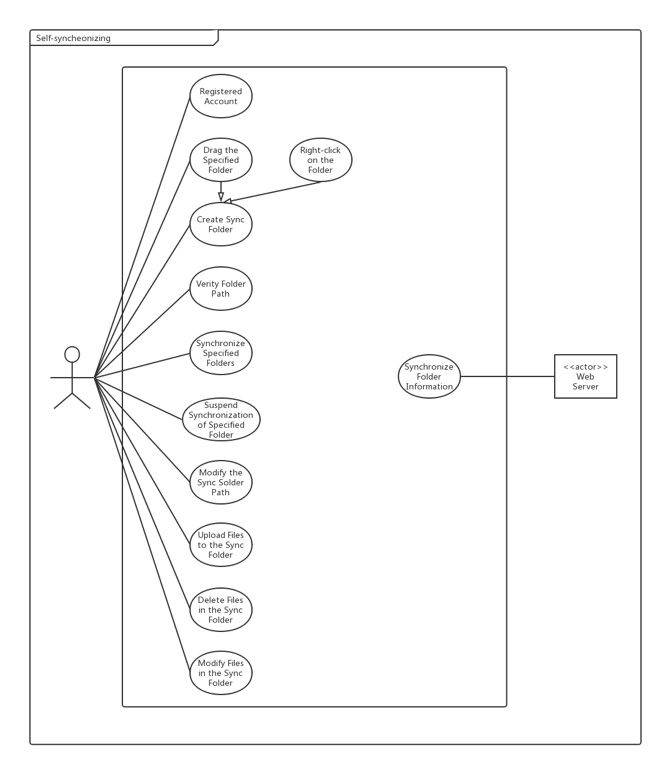
\includegraphics[width=12cm]{1.png}
		\caption{Use Case}
	\end{figure}
According to the UML, Group Paramount developed the Mobile Client UI and Desktop UI as in initial presentation. During the development process, Group Paramount found that some features could not be fully developed. Thus, the group decided to abandon some features and modify some features owing to time constraints. For example, combining the view file change record and modifying the file history version becomes a feature which is a file details function. In this function, users can view the created time of the file, version of the file and size of the file. Group Paramount deleted the pause synchronization function because it is useless for the current version of the application. Users can upload a new file to cover the old file if they want. Moreover, this biggest design objection is the team member's understanding of synchronizing. Some people believe that it is uploading to the server and showing with the same file list to users when users using Desktop Client or Mobile Client. Other people think that it is connecting to the file system. All files can automatically be synchronized to a server side in that folder and modified, edited files in this folder is different from other local folders. There are some very difficult parts of this problem.
\begin{enumerate}
	\item Whether the mobile client can access the system file.
	\item Whether the mobile client can online editing or online preview which needs to utilize third-party resources.
	\item What kind of files need to support online editing or online preview.
	\item In the Electron,  if the desktop client can access to the file system or not.
	\item In the Electron,  How long does it take for the whole team to complete this function( access to the file system and automatically synchronized to a server)? 
\end{enumerate}

According to these questions, Group Paramount did an investigation, it was found that on the mobile client, it is impossible to obtain the system folder as ROOT user. Moreover, for the function of online editing and preview, the group found that this function requires a lot of knowledge to learn how to connect with Word, how to save the editing content in real time and how to get the Word connection interface and use the native library(android studio) to build the UI without external library. Furthermore, The Electron is new to everyone in the Group Paramount, Team members need to spend a lot of time to learn how to use the Electron to connect with macOS or Windows. Based on the above analysis, Group Paramount decided to do synchronization in another way. Another way is the desktop client and the mobile client can sync files to the server and each client can see all files in the same account. In this way, Group Paramount needs to focus on fixing the conflict when two different clients uploading the same type of file to the server. With the development process, Group Paramount found the network speeds of different devices are different due to different environments. The conflict can be solved by the time of the end of the different upload file. The server will save the file is completed lately and another file is automatically saved as a historical version. This is a way to solve the conflict between uploading files at the same time. In addition, after completing the basic functions, Group Paramount found that it is also a useful feature to have time to do a user's ability to restore the historical version for a synchronization software, Group Paramount decided to add a recovery history version feature. However, due to the storage size of the server, Group Paramount decided to restore only the previous historical version. For the initial version of the application, Group Paramount has made the best efforts to design and complete the software in a limited time.

%%%%%%%%%%%%%%%%%%Part4%%%%%%%%%%%%%%%
\clearpage
\section{Implementation}

%%%%%4.1%%%%%
\subsection{Desktop: UI and Each Function}

%%4.1.1%%
\subsubsection{Refresh}
Refresh function displays all the files under the account. When the user clicks the Refresh button, the file list will display the file name, file size, and file creation date information of the corresponding file. For how to implement the query function, firstly, the system will monitor the Refresh button in real time. When the user clicks the button, the system will send an HTTP request to the server to get information about all the files under the account. When the system obtains the data in these JSON formats, it will perform the corresponding parsing process to obtain an array of file information. Next, the system traverses the array and displays the information for each file in the file list. For the challenge of implementing this function, the system needs to get the array by parsing the JSON data, and then extract the array in the array. The main function code as follows:
\begin{lstlisting}
const http = require('http');
var usernameha = localStorage.getItem("username");
console.log(usernameha);
http.get(
'http://teamparamount.cn:8080/Paramount/filesroot?username=' + usernameha, (resp) =>{
	let data = '';
	// A chunk of data has been recieved.
	resp.on('data', (chunk) =>{
		data += chunk;
	});
	// The whole response has been received. Print out the result.
	resp.on('end', () =>{
		var hhh = JSON.parse(data);
		var xxx = JSON.parse(data).info;
		var heh = JSON.parse(hhh.info);
		console.log(hhh);
		console.log(xxx);
		var trStr = '';
		for (var i = 0; i < heh.length; i++) {
			trStr += '<tr class="example">';
			trStr += '<td id="chebox0" ><input class="checkbox" type="checkbox" onclick="test(this);"></td>';            
			trStr += '<td contenteditable="true">' + heh[i].url + '</td>';
			trStr += '<td>' + heh[i].size + '</td>';
			trStr += '<td>' + heh[i].time + '</td>';
			trStr += '</tr>';
		}
\end{lstlisting}


Testing:
\\
\\
Our team use black-box testing method to test the refresh function.
\begin{figure}[htbp]
	\centering
	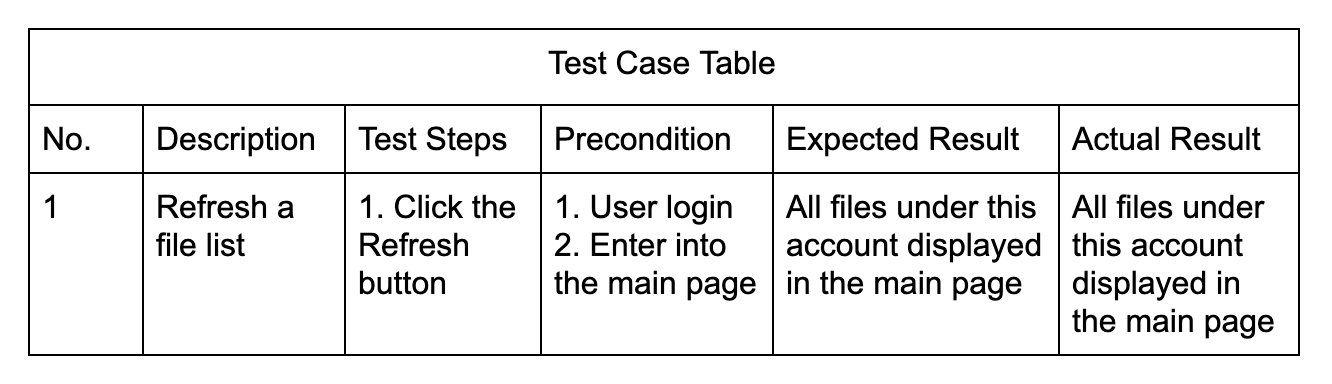
\includegraphics[width=12cm]{2.png}\\
	\caption{Test for Refresh Function}
\end{figure}

%%4.1.2%%
\subsubsection{Search}
Search function mainly provides users with the ability to quickly query one or some specified files under the account. When the user enters a specific file name in the specified file search box and then clicks the GO button, the corresponding file information is displayed in the file list. The search function has the following characteristics. Firstly, the user can perform a case-insensitive query which means the user does not have to care about the type of case. Secondly, the system can query all files with keyword input by the user. Thirdly, users can query all related files of a specific file type. For how to implement the query function, firstly, the system will monitor the GO button at any time. When the user clicks the button, the system will obtain the information input by the user in the query column, and send an HTTP request to the server to obtain all file information under the account. The system will then parse the JSON format data sent by the server, and then compare the data entered by the user with the file names of all corresponding files to find out all the files that the user needs. For the challenge of implementing this function, first, parsing the data containing the file type and file name into the corresponding file name. Second, the system needs to classify and discriminate the data input by the user. 
\\
\\
Testing:
\\
\\
Our team use black-box testing method to test the search function.
\begin{figure}[htbp]
	\centering
	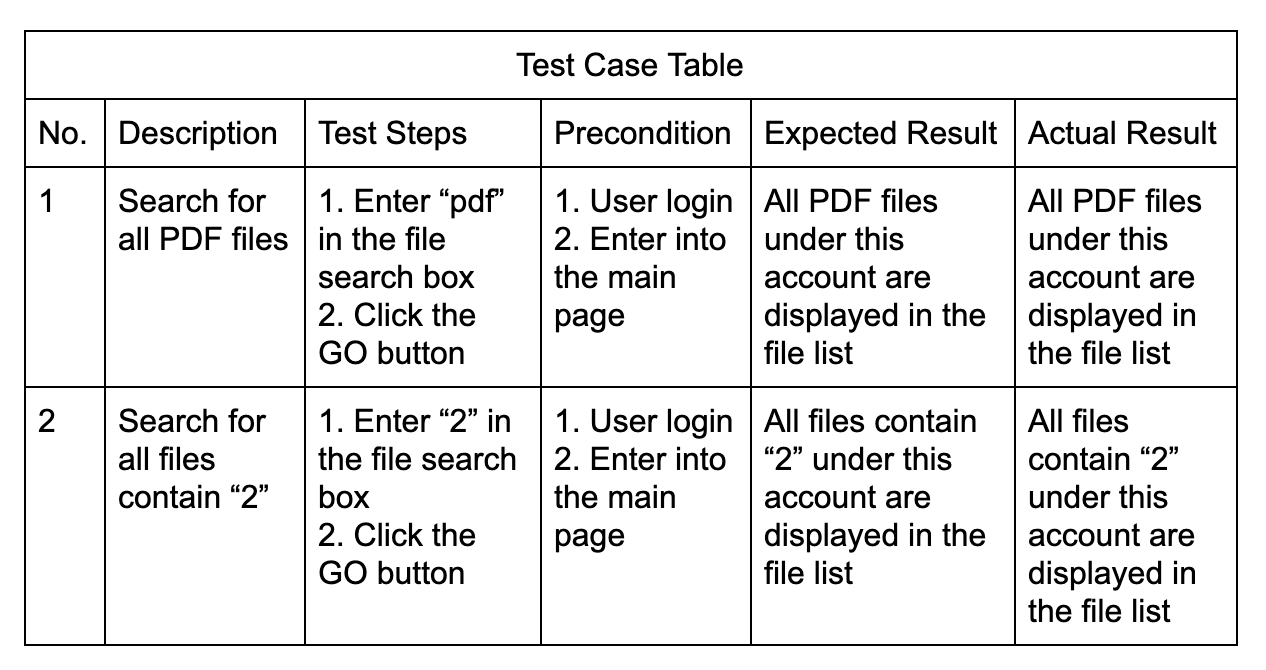
\includegraphics[width=12cm]{3.png}\\
	\caption{Test for Search Function}
\end{figure}

%%4.1.3%%
\subsubsection{Upload}
On upload file page, users could select a file upload to the server using form-data library\circled{3}. The file can be kinds of formats such as PDF, Word, Zip, jpg, and etc.. But on the desktop client, users could only upload one file at the same time. The step of uploading work starts to click the select file button. When users click the button, they can select a file and confirm it. Then the file name will show next to the button. If users want to change their selection, they could repeat the last step. Finally, users need to click the upload button to submit the file. During this progress, the progress bar starts work and on the right of the bar, the client will show the uploading speed and calculate the remaining time. Besides, users could use the cancel button to cancel the uploading. The main function code as follows:
\begin{lstlisting}
function UpladFile() {
	var fileObj = document.getElementById("file").files[0];
	var form = new FormData(); 
	form.append("file", fileObj); 
	xhr = new XMLHttpRequest();  
	xhr.open("post", "http://teamparamount.cn:8080/Paramount/upload", true); 
	xhr.onload = uploadComplete; 
	xhr.onerror =  uploadFailed; 
	xhr.upload.onprogress = progressFunction;
	xhr.upload.onloadstart = function(){
		ot = new Date().getTime();   
		oloaded = 0;
	};
	xhr.send(form);
}
\end{lstlisting}

Testing:
\\
\\
Our team use black-box testing method to test the upload function.
\begin{figure}[htbp]
	\centering
	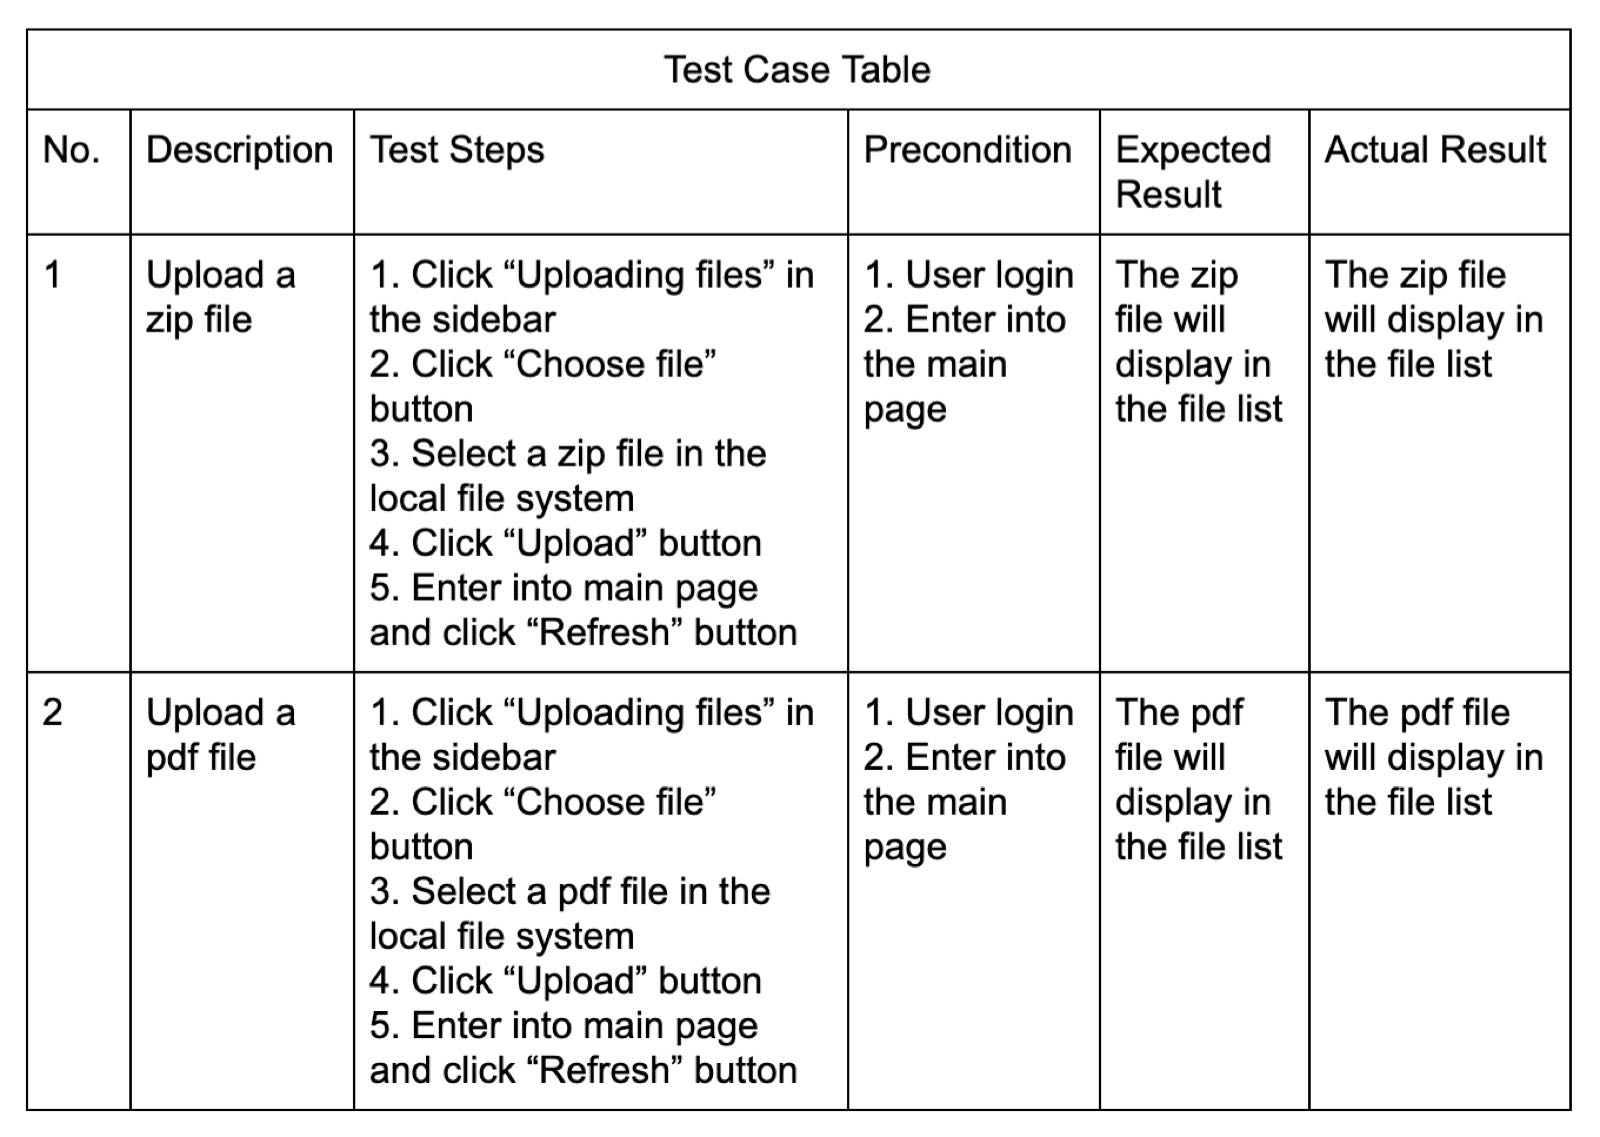
\includegraphics[width=12cm]{4.jpg}\\
	\caption{Test for Upload Function}
\end{figure}

%%4.1.4%%
\subsubsection{Delete and Download Page}
On delete page, users could select files which they do not need anymore to do the delete function. The first step of delete function is choosing file by selecting its checkbox. Then, users need to click “Delete” button to do delete function. When the “Delete” button is clicked, there is a message box to ask if the user really want to delete the item. When “Yes” button is clicked, the program selects the item which has been checked and then removes its whole line. After deleting it on the interface, the filename of the deleted item will be sent to the server, if the server accepts the deletion function successfully, then this item will be deleted in the database. 
\\
\\
The download page is using the same method to download a file. What the group wants to mention is during the designing and implementing the process, the biggest challenge is that when trying to send an HTTP request to the server, cross-domain issues arise when first use JavaScript to send HTTP requests if it is not in the Electron framework. However, the Group found that if using the JavaScript in the Electron, there is no cross-domain problem. Moreover, the electron is based on HTML, JavaScript, and CSS depending on node.js. The group found that the download function can use this library which is a node.js’s request HTTP\circled{4}. Using this request method, there is no any warnings or issues to send HTTP request. The main function code is as follows:
\begin{lstlisting}
//then, pick items which be checked
var items = document.getElementsByClassName('checkbox');
//set searching max length
var len = items.length;
//for loop search
for(var i = len-1; i >= 0; i--){
	//pick items which be checked
	var is_checked = items[i].checked;
	// delete item which checkbox has already be checked
	if (is_checked){
		//get lines which need to be deleted
		var divItem = items[i].parentNode.parentNode;
		//delete
		divItem.parentNode.removeChild(divItem);
		……
		var fileName = window.parent.str;
		//get deleted file's name
		const http = require('http');
		var usernameha = localStorage.getItem("username");
		http.get(
		"http://teamparamount.cn:8080/Paramount/delete?username=" + usernameha + "&url=" + fileName, (resp) =>{
			let data = '';
			// A chunk of data has been recieved.
			resp.on('data', (chunk) =>{
				data += chunk;
			});
			// The whole response has been received. Print out the result.
			resp.on('end', () =>{
				var hhh = JSON.parse(data);
				var xxx = JSON.parse(data).info;
				......
\end{lstlisting}


Testing:
\\
\\
Our team use black-box testing method to test the delete and download function.
\begin{figure}[htbp]
	\centering
	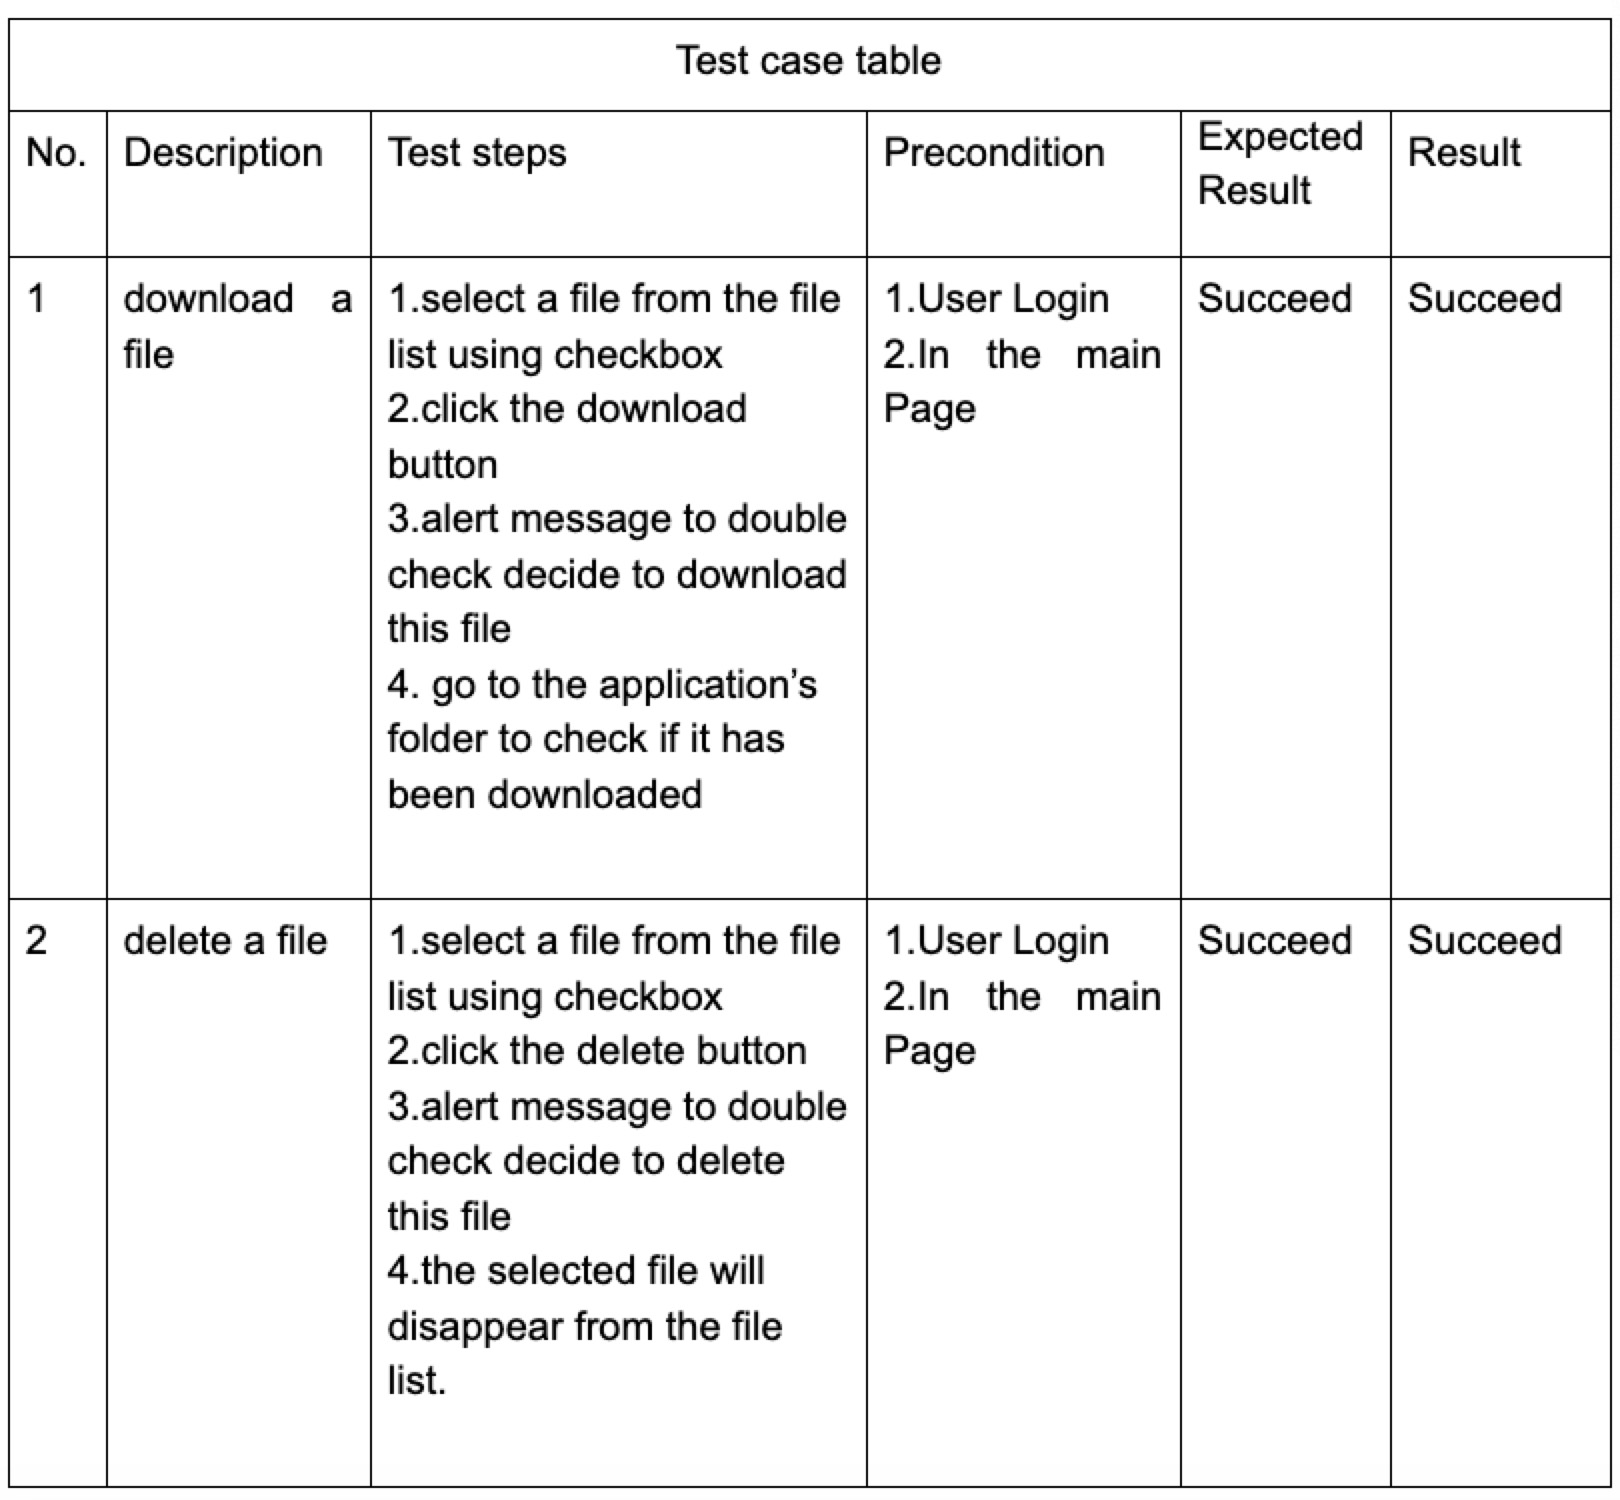
\includegraphics[width=12cm]{5.png}\\
	\caption{Test for Delete and Download Function}
\end{figure}
	
%%4.1.5%%
\subsubsection{Rename}
The Rename function is used to rename any file under this account. When the user selects the file that needs to be renamed, and then changes the file name of the corresponding file, and then clicks the Rename button, if the user renames successfully, the application will feedback a prompt for successful modification. If the user renames the same as a file name, the application will respond with a "the new file name is conflicted" prompt. The difficulty in implementing this function is how to get the old file name and the new file name separately. When a file is selected, the application will locate the file name cell in the table to read the file name. When the user clicks the Confirm Rename button, the application relocates to the cell specified in the table to read the modified file name. The main function code is as follows:
\begin{lstlisting}
var fileName1 = window.parent.str;
…...
var usernameha = localStorage.getItem("username");
http.get(
'http://teamparamount.cn:8080/Paramount/rename?username=' + usernameha + '&url=' + fileName1 + '&newUrl=' + fileName2, (resp) =>{
	let data = '';
	resp.on('data', (chunk) =>{
		data += chunk;
	});
	// The whole response has been received. Print out the result.
	resp.on('end', () =>{
		var hhh = JSON.parse(data);
		if (hhh.status == "success") {
			alert("Rename Succeed!");
		} else {
			alert(hhh.info);
		}
	});
}).on("error", (err) => {
	console.log("Error: " + err.message);
});
\end{lstlisting}

 
 Testing:
 \\
 \\
 Our team use black-box testing method to test the rename function.
 \begin{figure}[htbp]
 	\centering
 	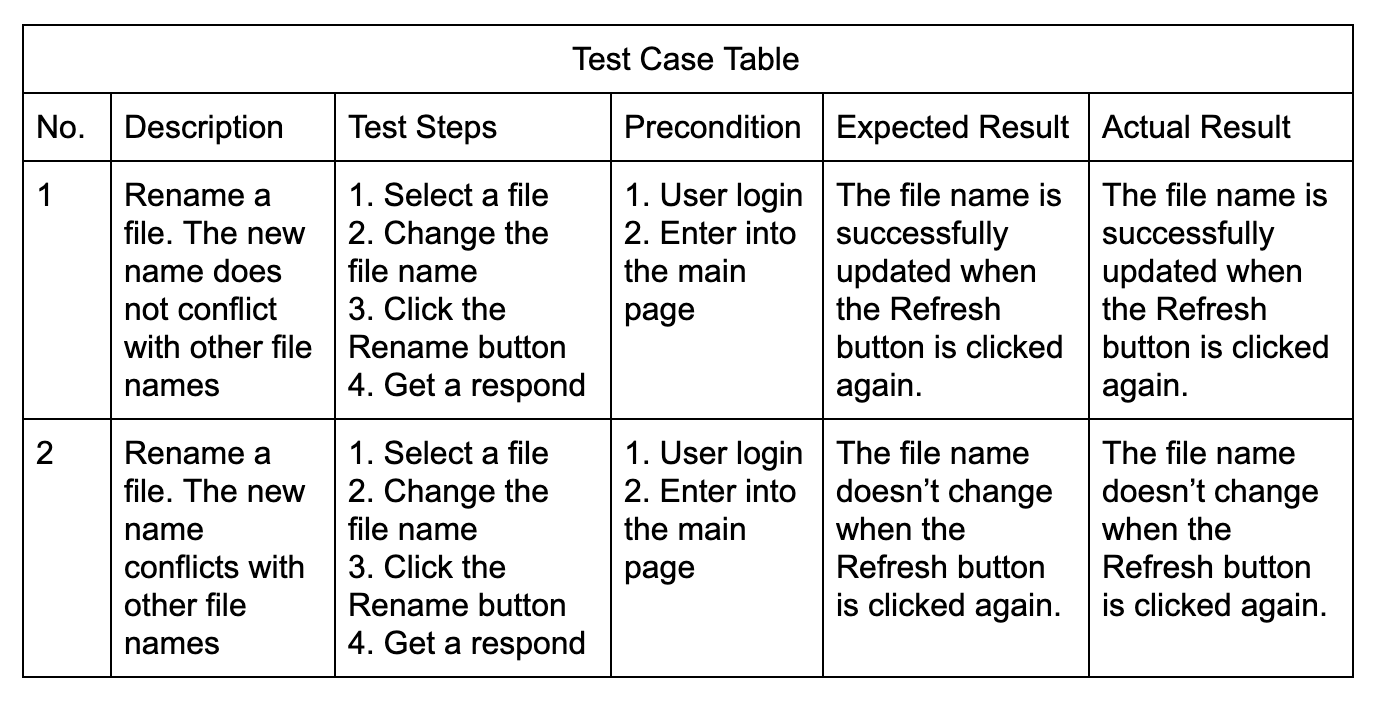
\includegraphics[width=12cm]{6.png}\\
 	\caption{Test for Rename Function}
 \end{figure}

%%4.1.6%%
\subsubsection{Revert}
When a file has multiple historical versions, Revert provides the user with the ability to restore the file to the previous historical version. The user selects a file and then clicks the Revert button to restore the version of the file. When the user chooses Revert to have no history version of the file, the application will prompt "can not revert first version". When the user selects a file that has been reverted once, the application will prompt "can not revert twice". The main function code is as follows:
\begin{lstlisting}
var usernameha = localStorage.getItem("username");
http.get(
'http://teamparamount.cn:8080/Paramount/revert?username=' + usernameha + '&url=' + fileName, (resp) =>{
	let data = '';
	// A chunk of data has been recieved.
	resp.on('data', (chunk) =>{
		data += chunk;
	});
	// The whole response has been received. Print out the result.
	resp.on('end', () =>{
		
		var hhh = JSON.parse(data);
		if (hhh.status == "success") {
			alert("Revert Succeed!");
		} else {
			alert(hhh.info);
		}
		......
\end{lstlisting}


 Testing:
 \\
 \\
 Our team use black-box testing method to test the revert function.
\begin{figure}[htbp]
	\centering
	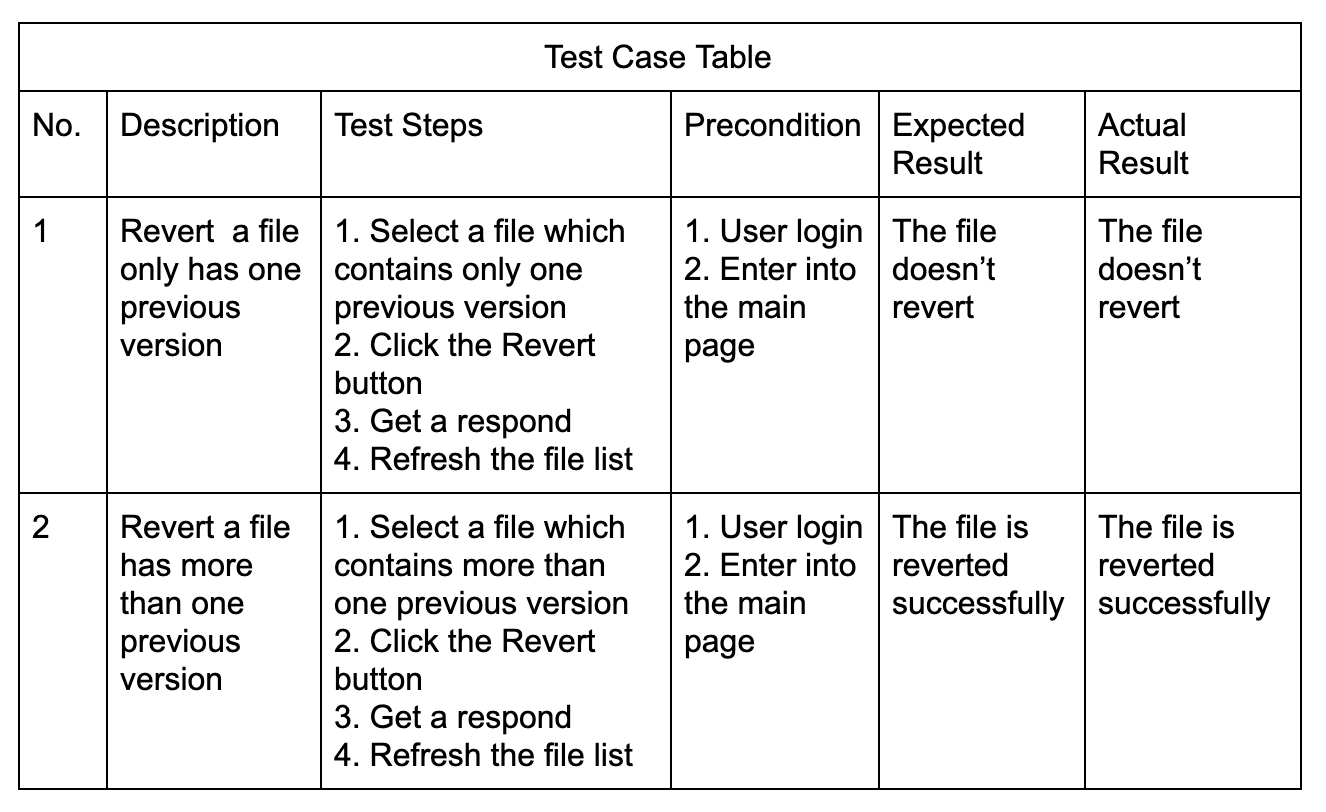
\includegraphics[width=12cm]{7.png}\\
	\caption{Test for Revert Function}
\end{figure}


%%%%%4.2%%%%%
\subsection{Mobile: UI and Each Function}
Based on the requirement of the project, the team decided to divide the mobile client into two components. The first component is the UI which is for to the users. The second component is the HTTP request and interfaces with the backend, such as how to send HTTP request to the server and how to get the response from the server.

%%4.2.1%%
\subsubsection{The UI Component}
\begin{itemize}
	\item 7 Activities Pages
	\item 3 fragments Pages
\end{itemize}

In this component, this group used fragments to form the main page/fragment, upload page/fragment, and user profile page/fragment, all of these pages/fragments in the Main\_Page.java. Users can jump to any page. The code is using to illustrate this function.

\begin{lstlisting}
@Override
public boolean onNavigationItemSelected(@NonNull MenuItem menuItem) {
	int id = menuItem.getItemId();
	if (id == R.id.home)
	{
		setFragment(homeFragment);
		return true;
	}
	else if (id == R.id.add)
	{
		setFragment(addFragment);
		return true;
	}
	else if (id == R.id.account)
	{
		setFragment(accountFragment);
		return true;
	}
	return false;
}
});
\end{lstlisting}


In order to help users to use the application more comfortable, this group added a lot of user-friendly design in each Activity Page, such as error checking in order to help users to check their mistakes when they type the username, password and so on.

%%4.2.2%%
\subsubsection{The HTTP Request and Interfaces with The Backend}
In this component, the mobile client needs to send an HTTP request to the server. This group looks for a lot of different HTTP request methods from a lot of materials. The group found that the Apache HttpClient has been removed from android API 23 6.0. Moreover, This traditional HTTP request method - HttpUrlConnection is considered by the group members to be a historical request method. The Group decided to use prevalent HTTP request method which is Okhttp request\circled{5} to write the HTTP request. In this project, upload function, download function, delete function, rename function, get file list function, file details function, and revert history version file function, all of these functions are using the Okhttp to send HTTP request. 
\\
\\
For HTTP request, This group decided to give some examples to illustrate different HTTP request methods such as POST and GET method as well as a response JSON file.

%%4.2.3%%
\subsubsection{Upload Function}
The upload function needs to send multipart or multi-data to the server. Firstly, The Okhttp request needs a request body including the upload file name, the type of file, the username and the location in the server. In addition, Using MaterialFilePicker\circled{6} to pick up a file.This is code from the Upload Page.

\begin{lstlisting}
public void run() {
	//select the file
	File f = new File(data.getStringExtra(FilePickerActivity.RESULT_FILE_PATH));
	// the type of file
	String content_type =  getMimeType(f.getPath());
	String file_path = f.getAbsolutePath();
	OkHttpClient client = new OkHttpClient();
	RequestBody file_body = RequestBody.create(MediaType.parse(content_type),f);
	// request the body
	RequestBody requestBody = new MultipartBody.Builder()
	.setType(MultipartBody.FORM)
	.addFormDataPart("file", f.getName(),
	RequestBody.create(MediaType.parse("multipart/form-data"), f))
	.addFormDataPart("username", username)
	.addFormDataPart("url","/")
	.build();
	Request request = new Request.Builder()
	.url("http://teamparamount.cn:8080/Paramount/upload")
	.post(requestBody)
	.build();
\end{lstlisting}


Each HTTP request is requested with the same request logic. The only difference is that the body of the request and request method will depend on the backend.

%%4.2.4%%
\subsubsection{Get File List Function}
The Get File List Function acquires all file by the current user from the server side and displays them to the user in a file list. This is using the GET method to send an HTTP request to the server.


\begin{lstlisting}
private void initFile(String username) {
	OkHttpClient okHttpClient = new OkHttpClient();
	Request request = new Request.Builder()
	.get()
	.url("http://teamparamount.cn:8080/Paramount/catalogroot?username=" + username)
	.build();
	Call call = okHttpClient.newCall(request);
	call.enqueue(new Callback() {
		@Override
		public void onFailure(Call call, IOException e) {
			System.out.println("fail to connect");
		}
		@Override
		public void onResponse(Call call, Response response) throws IOException {
			if (response.isSuccessful()) {
				......
\end{lstlisting}

From the code fragment, the group added the file logo to identify different type files by reading the file’s type. It should be mentioned here that the file information returned by the server is a JSON file, and the mobile client needs to parse the JSON file to obtain file information and identify the file type.

%%4.2.5%%
\subsubsection{File Detail Function}



From this code fragment, What the group would like to mention is also the JSON file. However, this JSON file includes multiple different variables which are size, type, version, and time. The mobile client used the array to parse this JSON file and show to users.

%%4.2.6%%
\subsubsection{MySharedPreferences}
SharedPreferences{[}2{]} is the easiest to understand data storage technology in Android. In fact, SharedPreferences handles a key-value (key-value pair) SharedPreferences commonly used to store some lightweight data. The MySharedPreferences.java is used stored the username for keeping the user login and sending HTTP request to the server. 
\\


This method/class is mainly used to read and save the correct user name entered by the user. It will be used to send HTTP request or show users information in the future.

%%4.2.7%%
\subsubsection{Testing}
For the testing part, the mobile client will use the black box testing and unit testing for the mobile client. This group decided to use the black box test to perform a functional simulation test on the mobile client. In the early and middle stages of research and development, this group draws the flow chart for each function. The basic style of the flow chart will be exemplified below.

\begin{figure}[htbp]
	\centering
	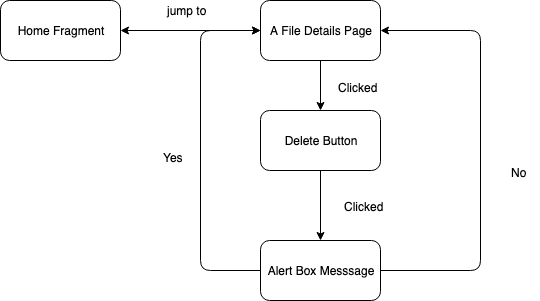
\includegraphics[width=12cm]{8.png}\\
	\caption{Flow Chart Sample}
\end{figure}

According to the specific functional flow chart, this group starts a black box test on each function to check for logical and functional errors. If a logic error occurs or the completion is extremely difficult, the group will adjust the logic or functional changes in time according to the relevant functions and schedules.
\\
\\
In the development process, the person in charge of each function will perform a self-function test, output the corresponding content in the terminal or prompt to jump to the corresponding page to test whether the function is correct. 
\\
\\
When performing self-tests, it is very effective to use a large number of system outputs corresponding values or to output the position where each program is performed. After the self-test is completed, the developer can comment out all the test statements and keep them in the program to find the source of the error when the developer perform unit testing later.
\\
\\
After all the basic functions of the mobile client were implemented, the group decided to test each function using unit testing. It is a test for correctness testing for program modules (the smallest unit of software design). The program unit is the smallest testable part of the application. In procedural programming, a unit is a single program, function, process, etc. For object-oriented programming, the smallest unit is the method, including the methods in the base class (superclass), abstract class, or derived class (subclass). For doing unit testing, this group draws an excel sheet to specify how many unit tests are in the mobile client, which is convenient for summarizing the test conditions of each function. The following table is a section taken from the complete excel sheet.

\begin{figure}[htbp]
	\centering
	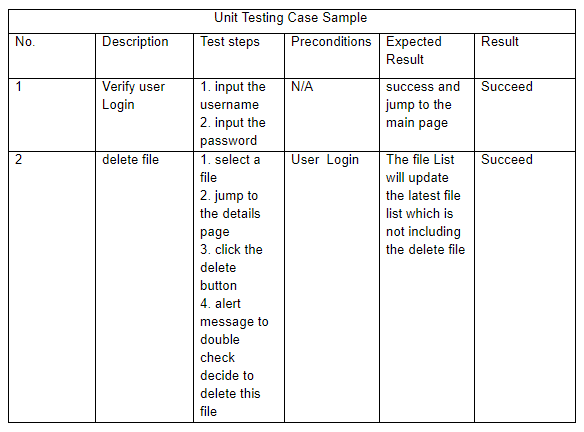
\includegraphics[width=11cm]{9.png}\\
	\caption{Unit Test Case Sample}
\end{figure}

According to the table, the mobile client is mainly designed and tested according to what functions each page has. The development process of the entire mobile client is basically to analyze the requirements, design functions, implement functions, test functions, and joint testing. For the joint testing, the group will discuss in the following pages.

%%%%%4.3%%%%%
\subsection{Back-end}

%%4.3.1%%
\subsubsection{Design}
The back-end server uses Java language to build it, based on the Spring Boot{[}3{]} Framework. Spring Boot\circled{7} is a project created on the top of  Spring Framework. It provides a simpler and faster way to set up, configure and run both web-based and straightforward application. Both desktop and mobile clients can request the services through HTTP requests and get responeses in Json format which created by fastJson\circled{8}. According to this fact, the web-based server is quite useful and powerful. The specific request document can access on GitHub.  
\\
\\
The back-end application contains 34 Java classes which have more than two thousand lines source code. The chosen database is MySQL and the application is run on the Amazon EC2 server. The whole project uses 5-tier architecture. Please refer to Figure 10 (see next page) for the architecture diagram.
\\



The client tier contains mobile and desktop clients which will request the service from the server remotely via the HTTP request.
\\
\\
The presentation tier consists of the different controller, these components enforce the interaction sequencing. The different requests of the service have a different controller which can correct invoke the underlier components. 
\\
\\
The business tier is the most complex tier, which consists of components that provide the business logic for the application. In the business tier, it contains 4 individual components corresponding to the different domain logic, and the most important one is the file business component.
\\
\\
The integration tier contains database interfaces, and these allow the server system can access to the MySQL database to store the relevant data.
\\
\\
The resource tier consists of MySQL database and Amazon EC2 cloud server. The MySQL database has tables to save the user information and the record of the uploaded file. Due to the efficient usage of the system, the files saved in the server instead of saving in the database. In this scenario, the files will save in the folders independent for each user.

\begin{figure}[htbp]
	\centering
	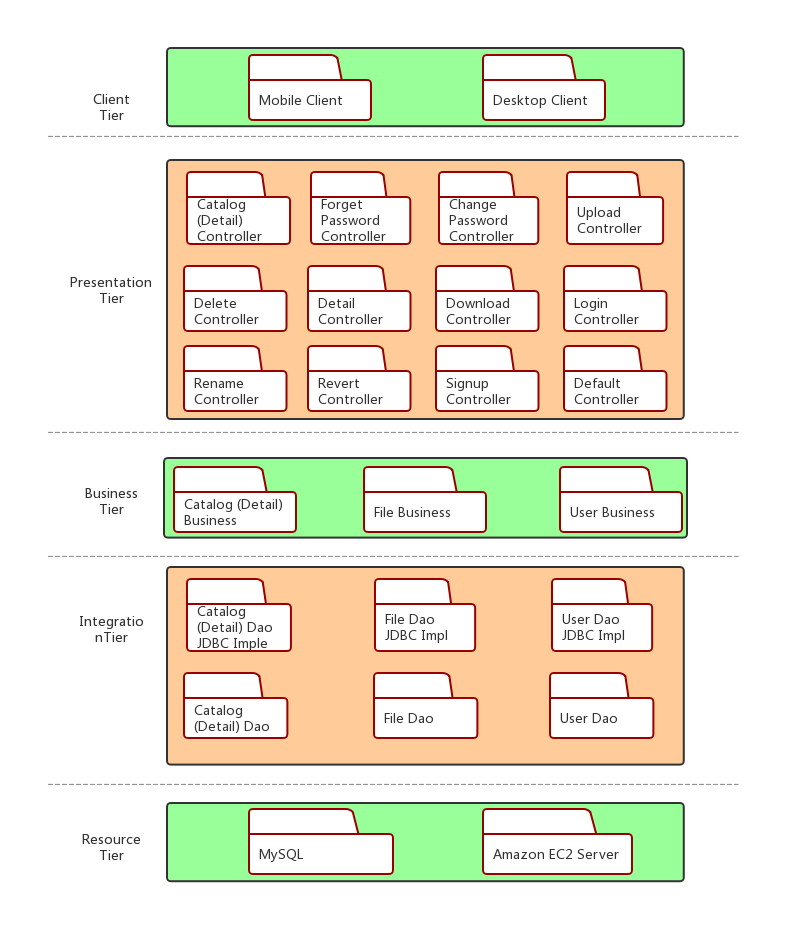
\includegraphics[width=11cm]{10.png}\\
	\caption{Architecture of The Server}
\end{figure}

%%4.3.2%%
\subsubsection{Implementation}
The attached are some specific implementations of essential functions, such as upload, download, revert, delete and rename.
\\
\\
This is the function of upload, it checks the conflict of two clients are upload the same name file at the same time and save the original file to the specific folder on the server.

\begin{lstlisting}
public String upload(String username, MultipartFile file, String url) {
	FileDao fd = new FileDaoJDBCImpl();
	String result = null;
	String checkurl;
	…… 
	else {
		checkurl = file.getOriginalFilename();
	}
	Boolean flag = fd.checkFile(username, checkurl);
	if (flag == true) {
		if (fd.isLock(username, checkurl) == true) {
			result = JSONUtils.getJSONString("fail", "uploading conflict");
		}
		else {
			fd.lock(username, checkurl);
			result = addUpdatedFile(username, file, url);
			fd.updateFile(username, checkurl);
			fd.unlock(username, checkurl);
		}
	}
	else{
		result = addNewFile(username, file, url);
	}
	return result;
}
\end{lstlisting}

The download function is a straightforward function that through the necessary HTTP request and the requested file as the attachment of the HTTP Get request.


\begin{lstlisting}
@RequestMapping(value = "/download", method = RequestMethod.GET)
public String download(HttpServletResponse response,
@RequestParam("username") String username,
@RequestParam("url") String url) {
	…...
	File file = new File(filePath);
	if (file.exists()) {
		response.setHeader("content-type", "application/octet-stream");
		response.setContentType("application/octet-stream");
		response.setHeader("Content-Disposition", "attachment;filename=" + file.getName());
		
		byte[] buffer = new byte[1024];
		FileInputStream fis = null;
		BufferedInputStream bis = null;
		try {
			fis = new FileInputStream(file);
			bis = new BufferedInputStream(fis);
			OutputStream os = response.getOutputStream();
			int i = bis.read(buffer);
			while (i != -1) {
				os.write(buffer, 0, i);
				i = bis.read(buffer);
			}
		}
		…… 
		return null;
	}
\end{lstlisting}

The revert can change the file to the last version, because of the server save at most two versions of the same file. If the revert function invokes, the latest file will be deleted, based on this implementation that the function can prevent clients unlimited revert to some extent.


\begin{lstlisting}
public String revert(String username, String url) {
	String result = null;
	String filePath;
	FileDao fd = new FileDaoJDBCImpl();
	Integer vi = fd.getFileVersion(username, url);
	if (vi == 0) {
		result = JSONUtils.getJSONString("fail", "can not revert first version");
	}
	else {
		String storedName = url;
		…… 
		File file = new File(filePath);
		if (file.exists() == false) {
			result = JSONUtils.getJSONString("fail", "can not revert twice");
		}
		else {
			try {
				FileInputStream fis = null;
				fis = new FileInputStream(file);
				FileChannel fc = fis.getChannel();
				SimpleDateFormat ft = new SimpleDateFormat("yyyy-MM-dd HH:mm:ss");
				String time = ft.format(file.lastModified());
				File deleteFile = new File(ROOT_PATH + username + pre + nowVersion + post);
				if (fd.revert(username, storedName, fc.size(), time) && deleteFile.delete()) {
					result = JSONUtils.getJSONString("success", "");
				} else {
					result = JSONUtils.getJSONString("fail", "unknown reasons");
				}
			} catch (IOException e) {
				result = JSONUtils.getJSONString("fail", e.getMessage());
			}
		}
	}
	return result;
}
\end{lstlisting}

The delete function will delete the specific file, if the saved file not only the one version, this function will delete  both version and delete the record in the database.


\begin{lstlisting}
public String delete(String username, String url) {
	String result = null;
	FileDao fd = new FileDaoJDBCImpl();
	Integer vi = fd.getFileVersion(username, url);
	Boolean flag1 = fd.checkPreDic(username, url);
	Boolean flag2 = fd.checkPreFile(username, url);
	if (flag1 && flag2) {
		flag1 = fd.delectInFile(username, url);
		flag2 = fd.delectInDir(username, url);
		if (flag1 && flag2) {
			…… 
			String delteFile;
			delteFile = ROOT_PATH + username + pre + nowVersion + post;
			File file = new File(delteFile);
			file.delete();
			delteFile = ROOT_PATH + username + pre + otherVersion + post;
			file = new File(delteFile);
			if (file.exists()) {
				file.delete();
			}
			result = JSONUtils.getJSONString("success", "");
		}
		else {
			result = JSONUtils.getJSONString("fail", "unknown reasons");
		}
	}
	else {
		result = JSONUtils.getJSONString("fail", "the directory may not empty");
	}
	return result;
}
\end{lstlisting}
The rename function can change the file name (both version) saved on the server, but there is a little bug will be introduced. That the last change time of the file will be changed and it will not show on the details of the file until the revert function called. 

\begin{lstlisting}
public String rename(String username, String url, String newUrl) {
	String result = null;
	File file = new File(newUrl);
	String name = file.getName();
	if (name.contains(".") == false) {
		result = JSONUtils.getJSONString("fail", "the type of file if missed");
	}
	else {
		…...
		if (fd.checkFile(username, newUrl) == true) {
			result = JSONUtils.getJSONString("fail", "the new file name is conflicted");
		} else {
			if (fd.rename(username, url, newUrl)) {
				…...
				File oldFile = new File(oldPath);
				if (oldFile.renameTo(new File(newPath))){
					result = JSONUtils.getJSONString("success", "");
				}
				else {
					result = JSONUtils.getJSONString("fail", "rename error");
				}
				oldFile = new File(oldPath1);
				if (oldFile.exists()) {
					if (oldFile.renameTo(new File(newPath1)) == false) {
						result = JSONUtils.getJSONString("fail", "rename error");
					}
				}
			} else {
				result = JSONUtils.getJSONString("fail", "unknown reaseons");
			}
		}
	}
	
	return result;
}
\end{lstlisting}


%%4.3.3%%
\subsubsection{Testing}
The primary methods for the server to test the correctness and effectiveness are via local tests and client requests. When each function completed, the local unit test will check the basic usability of the feature. Because the server is a kind of web-based application, most of the tests can use a browser to verification. Check the consistency between the document and the real representation.
\\
\\
The majority of the tests are performed by the clients' requests. If the clients could always receive the expected response, during the developing process, the performance of the server is the same as expected. Both the desktop client and mobile server have the same back-end server. In this scenario, the request methods and responses are the same, only different display forms. The ways to check the server correctness can access through the previous chapter.
\\
\\
When some interfaces may have some defects and detected by the clients, the developer will change the behaviour of the function and do the regression tests. Through this method, it can ensure amended the defects do not turn the main feature in another direction.

%%%%%4.4%%%%%
\subsection{The Joint Testing}
The joint testing focus on desktop client and mobile client. This testing mainly helps the group to test if there are any bugs when two clients are operating at the same time. The group decided to test the two clients all the same functions and use the unit testing method. The most significant challenge for joint testing is the synchronization when two clients upload the same name and the same type of file. With the development process, Group Paramount found that there are a lot of factors can influence the synchronization in real life, such as the Internet speed, the file size, the device CPU and so on. According to these situations, The server will save the file recently and another file will be automatically saved as a historical version. This is a way which the group how to resolve conflicts in uploading files. With the testing of many different types of files, the group did not find any problems so far.


%%%%%%%%%%%%%%%%%%%Part5%%%%%%%%%%%%%
\clearpage
\section{Teamwork}
The team was born on 18th January 2019 and named as Paramount. On the first day of the team formation, the team has a short meeting to discuss how the team will work in the future. After the meeting, the team decided that the group will have two meetings every week. One is on Wednesday, which held in the Waterloo library group study room. The meeting will discuss the completion of the work last week and what should everyone do in next week. Another meeting is online meeting every Sunday night. This meeting focus on team member’s problems. Everyone give their problem during the process and all team will discuss how to solve the problem.
\\
\\
In the whole development process, the team uses a lot of tools to facilitate group work. There are main tools that the team used in daily work as follows. On meeting and records aspect, it includes Trello, QQ, Wechat, TeXstudio, Google drive, and Teamviewer. On coding developing aspect, it includes GitHub, draw.io, Android Studio, Mockplus, Genymotion, Brackets, and Atom. Trello is a good tool to record duties and it will alert you to make every member do it as soon as possible. QQ and Team Viewer are excellent tools used for the online meeting. People not only could see others face on their screen but also could show desktop to others. It is convenient for an online meeting. Because the team crews are all Chinese and we all use Wechat. So Wechat becomes to the daily communication tool. TeXstudio is used to edit the report. Google Drive is another brilliant tool which makes several people edit one Word document at the same time and people can share the document easily. According to the project requirements, all works have to pull on GitHub. The programmer could save their code on different repositories. Besides, people could give comments on own codes as well as learn other codes and provide some suggests. It provides the team with a good platform to study and communication. Draw.io is used to draw Use case and class diagram. It makes the team easy to design the project at the beginning. The team decided to design the desktop client and Android client. So the team needs an Android integrated development environment(IDE) and Android Studio is the best choice. Mockplus is a tool to design the Android prototype. This is easy to learn and have a perfect function. Genymotion is an Android emulator which make us test the project. Brackets and Atom are both source code editor to build the desktop client. Though these tools, group project could facilitate efficiently.
\\
\\
Then, there are some brevity demonstrations of meeting records which show the process of the development.
\\
\\
\textbf{20th January 2019:}
\\
\\
Giving the name of the team. Temporary choosing Android and Mac OS desktop as a client. According to the calendar, deciding what should do before the intermediate presentation. Before next Wednesday duty is according to the project requirements everyone draws a use case diagram.
\\
\\
\textbf{23rd January 2019:}
\\
\\
According to everyone’ s use case diagram, the group decide the final use case diagram and draw it. Dividing the whole team into two part, three in charge of Android UI design and the other in charge of Mac client UI design. Everyone should learn how to use GitHub.
\\
\\
\textbf{30th January 2019:}
\\
\\
Because all team members are not familiar with Swift language and members do not have enough time to learn it, the team adjust Mac OS client to Electron + Node.js as the desktop client. Next week duty is to improve the client UI and write the initial report. Two of the team members should learn how to use Latex to edit the report.
\\
\\
\textbf{6th February 2019:}
\\
\\
On this meeting, the group checks the desktop and Android UI and final inspect the report. Besides, the team members allocate everyone’ s task in the initial presentation. Because the presentation is on two days later, crews have to prepare slides and practice presentation together.
\\
\\
\textbf{13th February 2019:}
\\
\\
After the initial presentation, the team has a short break. On this meeting, the group assigns next week work which includes setting up the database, server and coding the software function.
\\
\\
\textbf{6th March 2019:}
\\
\\
These three weeks, the main duty is coding the function of the program. Up to now, the group already have finished all basic function such as login in, sign in, upload files, refresh the home page, delete existing files, download files both on the desktop and Android client.  Then the team wants to try to add more function such history records and so on. Most important work of next week solves the conflicts.
\\
\\
\textbf{13th March 2019:}
\\
\\
The main task of this meeting is to distribute the final report to write. There are seven parts of the report. Every team member in charge of one part except the implementation part and then writing part four together. The desktop client still needs to improve functionality.
\\
\\
\textbf{20th March 2019:}
\\
\\
On this meeting, the whole team check the draft report and find the problem.
Then, everyone chooses one part to prepare their presentation. Two of the team members are in charge of typesetting the final report through Latex.

%%%%%%%%%%%%%%%%%Part6%%%%%%%%%%%%%%
\clearpage
\section{Evaluation}
In terms of the whole development process, the majority of the steps are quite good. Especially every team members try to enjoy the entire process. At the very beginning, some members have limited programming skills even some of them have not any programming experience at the undergraduate period, but they are doing their best to learn more knowledge about relevant to the project. The most of advantage for this project is to let everyone involved in this teamwork and gain advanced computing skills. After this module, each member gets the ability to build a software system and collaborate with a team. The crews cooperate very well, the meetings of the group are correctly formed,  nobody escapes any meeting at all whatever online or physically. In the developing process, when meeting the puzzles, each one tries to solve the problem to help the team participant. During this process, everyone involved will get the benefits from it, either enhance their ability or learn the new knowledge. The main profit of this Group Project module is to let each team member improve their programming skills. 
\\
\\
The aspect of implementation is the weakness of the group, due to the time limit, the group has not enough to learn many technologies of this project. So we decided the group to some sub-groups. Kexin Lin primarily takes the response to the mobile platform. Kunxiang Jin mainly takes charge of the backend of the system. Bo He, Zhipeng Qi, Yu Zhu, and Yiran Xu present the desktop system, the most of new knowledge focuses on the desktop part. In the beginning, the group decided to use Swift to build a MacOS system, but the language restriction and there is not enough information on the web, the decision was changed to use Electron to make the sub-system (desktop).  The experience is the most significant limitation for this group, because of the most of knowledge is remained on the theoretical level, there are still many gaps between theories and reality. Due to the expectation of the process, the Paramount group wants to make each one to get the comprehensive development. Although everyone is taking part in separate parts of the system, they need to learn the necessary skills of each part of the system. Learning to much staff is a time-consuming way, but it is useful for members in future careers.
\\
\\
At the beginning of the life cycle, the team spent to much time on deciding which tools will use and the presence of the project. The first two weeks on learning how to use Swift to build a desktop platform, but this technology not used in the real development process, so this is not a better way, even wasting time. If the project can start again, the team will try the best to analysis at first, to investigate the background and find the most proper way to build the system. 
\\
\\
Even Git is a powerful tool which can be used in the software developing process. The Paramount team did not suitably use this tool. The truth that only a part of crews used Git before is undeniable, so when used the pull request future, there are seldom comments, even no comments. No comments mean the code changes may contain some errors, but no one reviews it. From the email of the lecture, that at least ten comments even fifty or more are relatively common in the real usage.
\\
\\
As proposed, the team will build a system to synchronize a local folder. When the group wants to implement it, this is hard to come true. So the implementation was changed to save the files on the cloud, and each operation of the saved data is via the mobile or desktop application. This implementation is not as expected. According to the ability of the group, the changes are necessary.
\\
\\
The teamwork methods of our group are using git and the Internet.  The git is a mainstream version control tools,  by using this tool, the team members can quickly get the latest version of the whole project. There are meetings for the meet physically and remotely, through the meeting team members have the chance to discuss the problem with each other — this always a useful way to solve the problems. At the meantime,  it is an excellent way to track the progression, the coordinator or members can check whether ahead or behind schedule.
\\
\\
Through the whole project, everyone involved in this group enhance the computing abilities and the ability that cooperate with other people. Try to learn some entirely new knowledge, and correctly use these technologies. In nine weeks, build a multi-client and central server application. The system is not the best even not the better system, but it is the concentration of effort and learning of team member.  

\clearpage
%%%%%%%%%%%%%%%%Part7%%%%%%%%%%%%%%%

\section{Peer Assessment}
In this project, all members are allocated the total marks averagely (each person get 16.66 points).


%%%%%%%%%%%%%%%Part8%%%%%%%%%%%%%%%%

\section{References}
\begin{enumerate}[label={[}\arabic*{]}]
	\item Electron Tutorial,{[}online{]}, Available at:
	\\
	https://electronjs.org/docs/tutorial/quick-start
	\\
	(accessed on 30.01.2019)

	\item How to store data locally in an Android app,{[}online{]}, Available at:
	\\
	https://www.androidauthority.com/how-to-store-data-locally-
	\\
	in-android-app-717190/ (accessed on 05.02.2019)
	
	\item Spring Boot Tutorial,{[}online{]}, Available at:
	\\
	https://www.tutorialspoint.com/spring\_boot/index.htm
	\\ 
	(accessed on 09.02.2019)
	
\end{enumerate}

\section{External Libraries}
\begin{enumerate}[label=\circled{\arabic*}]
\item jQuery: https://jquery.com
\item bootstrap: https://getbootstrap.com
\item form-data library: https://www.npmjs.com/package/form-data
\item node.js'request HTTP: https://nodejs.org/api/https.html
\item OkHTTP: https://square.github.io/okhttp
\item MaterialFilePicker: https://github.com/nbsp-team
\item Spring Boot: https://spring.io/projects/spring-boot
\item fastJson: https://github.com/alibaba/fastjson
\end{enumerate}


\end{document}